\documentclass[12pt,a4paper,onecolumn]{article}

%%%%%%%%%%%%%%%%%%%%%%%%%%%%%%%%%%%
%          				PACKAGES  				              %
%%%%%%%%%%%%%%%%%%%%%%%%%%%%%%%%%%%

\usepackage[margin=1in]{geometry}
\usepackage{authblk}
\usepackage{caption}
\usepackage[utf8]{inputenc}
\usepackage{amsfonts}
\usepackage{a4wide,graphicx,color}
\usepackage{amsmath}
\usepackage{amssymb}
\usepackage[table]{xcolor}
\usepackage{setspace}
\usepackage{booktabs}
\usepackage{dcolumn}
\usepackage{rotating}
\usepackage{color,soul}
\usepackage{threeparttable}
\usepackage[capposition=top]{floatrow}
\usepackage[labelsep=period]{caption}
\usepackage[spanish]{babel}
\usepackage{subcaption}
\usepackage{lscape}
\usepackage{pdflscape}
\usepackage{multicol}
\usepackage[bottom]{footmisc}
\setlength\footnotemargin{5pt}
\usepackage{longtable} %for long tables
\usepackage{graphicx}
\usepackage{enumerate}
\usepackage{units}  %nicefraction
\usepackage{placeins}
\usepackage{booktabs,multirow}
%% BibTeX settings
\usepackage{natbib}
\bibliographystyle{apalike}
%\bibliographystyle{unsrtnat}
\bibpunct{(}{)}{,}{a}{,}{,}


%% paragraph formatting
\renewcommand{\baselinestretch}{1}


% Defines columns for tables
\usepackage{array}
\newcolumntype{L}[1]{>{\raggedright\let\newline\\\arraybackslash\hspace{0pt}}m{#1}}
\newcolumntype{C}[1]{>{\centering\let\newline\\\arraybackslash\hspace{0pt}}m{#1}}
\newcolumntype{R}[1]{>{\raggedleft\let\newline\\\arraybackslash\hspace{0pt}}m{#1}}

\usepackage{comment} %to comment entire sections



\usepackage{bbold} %for indicators

\setcounter{secnumdepth}{6}  %To get paragraphs referenced 

\usepackage{titlesec} %subsection smaller
\titleformat*{\subsection}{\normalsize \bfseries} %subsection smaller
%\usepackage[raggedright]{titlesec} % for sections does not hyphen words


\usepackage[colorlinks=true,linkcolor=black,urlcolor=blue,citecolor=blue]{hyperref}  %Load last
%% markup commands for code/software
\let\code=\texttt
\let\pkg=\textbf
\let\proglang=\textsf
\newcommand{\file}[1]{`\code{#1}'}
\newcommand{\email}[1]{\href{mailto:#1}{\normalfont\texttt{#1}}}
\urlstyle{same}

%%%%%%%%%%%%%%%%%%%%%%%%%%%%%%%%%%%
%     			TITLE, AUTHORS AND DATE    			  %
%%%%%%%%%%%%%%%%%%%%%%%%%%%%%%%%%%%
%% Title, authors and date

\title{PS1 }

\author{Catalina Leal Rojas, Lucas Daniel Carrillo Aguirre, Lucas Eduardo Veras Costa, Maria Paula Basto Lozano} 
\date{\today}

\begin{document}



\maketitle

\thispagestyle{empty} % Leaves first page without page number

%



%%%%%%%%%%%%%%%%%%%%%%%%%%%%%%%%%%%
%    DOCUMENT    		          %
%%%%%%%%%%%%%%%%%%%%%%%%%%%%%%%%%%%




\section{Introduction} \label{sec:intro}

Here you have to position your paper, remember RAP:
\begin{enumerate}
    \item R: research question
    \item A: your answer
    \item P: positioning in the existing literature
\end{enumerate}

\section{Literature Review}

A couple of things here. First, I prefer not to have a separate section, I think it's better to have it as part of the introduction, where you can cite the papers to position yours, and also in contrasting your contribution. You can also fold this when discussion your results, so you can compare/contrast with the existing literature


If you decide to have a separate section, please be careful in relating it to your research. I encurage you to read and follow \cite{nikolov2020writing}\footnote{This is available in the \href{https://ignaciomsarmiento.github.io/teaching/Tesis.html}{course website}} excellent advice:

\begin{quote}
    {\it ``Do not title your literature review section ``literature review''! It is a bit sophomoric. Instead, integrate your discussion of previous literature under the common thread of previous work as it relates to your main thesis.  For example if your paper is ``Do Traditional Institutions Constrain Female Entrepreneurship?'' you might want to call your literature review ``Gender norms in India''. In other words, tell your readers what is in the section...''} \citep{nikolov2020writing}
\end{quote}



\section{Data}

\section{¿Trabajos semejantes pagos semejantes?}

En esta sección analizaremos la relación entre ingresos y género femenino. 
En primer lugar, es importante discutir qué medida de ingreso utilizar. 
La base de datos de la GNIH incluye diversas medidas, como ingreso por primas monetarias, ingreso mensual, ingreso usual en el mes e ingreso efectivo en el mes, entre otras. 

En los estudios que analizan la brecha salarial entre hombres y mujeres, es común emplear el ingreso por hora, ya que permite aislar el efecto de las horas trabajadas en el mes, lo cual podría sesgar los resultados. 
Asimismo, suele utilizarse la variable de ingreso en logaritmos, lo que mejora la interpretabilidad del coeficiente estimado, que pasaría a representar cuánto impacta, en términos porcentuales, una unidad adicional de la variable independiente sobre el ingreso. 

También es importante señalar que nos interesa comparar únicamente a hombres y mujeres que trabajan. 
Por lo tanto, el análisis se centra en los individuos ocupados de la muestra.

Inicialmente estimamos el siguiente modelo:

\begin{equation}
\log(\omega) = \beta_0 + \beta_1 Female + u 
\label{eq_inc}
\end{equation}


\begin{table}[!htbp] 
\centering    
\caption{Resultados del modelo incondicional}    
\label{cuadro_inco}  
\resizebox{\textwidth}{!}{%
\begin{tabular}{@{\extracolsep{5pt}}lccccc}  
\\[-1.8ex]\hline  
\hline \\[-1.8ex]   
& \multicolumn{5}{c}{\textit{Variable dependiente:}} \\  
\cline{2-6}  
\\[-1.8ex] & log(ysalarym) & log(ysalarymha) & log(yingLabm) & log(ytotalm) & log(ytotalmha) \\  
\\[-1.8ex] & (1) & (2) & (3) & (4) & (5)\\  
\hline \\[-1.8ex]   
female & $-$0.149$^{***}$ & $-$0.045$^{***}$ & $-$0.147$^{***}$ & $-$0.238$^{***}$ & $-$0.090$^{***}$ \\    
& (0.015) & (0.015) & (0.015) & (0.015) & (0.014) \\    
& & & & & \\   
Constant & 13.977$^{***}$ & 8.641$^{***}$ & 14.088$^{***}$ & 13.981$^{***}$ & 8.667$^{***}$ \\    
& (0.011) & (0.010) & (0.011) & (0.010) & (0.009) \\    
& & & & & \\  
\hline \\[-1.8ex]  
Observaciones & 9,892 & 9,892 & 9,892 & 14,764 & 14,764 \\  
R$^{2}$ & 0.010 & 0.001 & 0.009 & 0.018 & 0.003 \\  
R$^{2}$ ajustado & 0.010 & 0.001 & 0.009 & 0.017 & 0.003 \\  
Error estándar residual & 0.751 (df = 9890) & 0.721 (df = 9890) & 0.762 (df = 9890) & 0.889 (df = 14762) & 0.832 (df = 14762) \\  
F Statistic & 97.364$^{***}$ (df = 1; 9890) & 9.559$^{***}$ (df = 1; 9890) & 91.422$^{***}$ (df = 1; 9890) & 263.841$^{***}$ (df = 1; 14762) & 43.342$^{***}$ (df = 1; 14762) \\  
\hline  \hline \\[-1.8ex]  
\textit{Nota:}  & \multicolumn{5}{r}{$^{*}$p$<$0.1; $^{**}$p$<$0.05; $^{***}$p$<$0.01} \\  
\end{tabular}  
} % cierre de resizebox
\end{table}
El Cuadro \ref{cuadro_inco} presenta los resultados de la estimación por mínimos cuadrados ordinarios utilizando diversas medidas de ingreso. 
$ysalarym$ corresponde al ingreso nominal de la ocupación principal, $ysalarymha$ al salario por hora de la ocupación principal, $yingLabm$ al ingreso proveniente de todas las ocupaciones, $ytotalm$ al ingreso total proveniente de ocupaciones e ingresos independientes, y $ytotalmha$ al ingreso total de ocupaciones e independientes medido por hora.

Los resultados muestran evidencia de que las mujeres ganan menos que los hombres. Aunque existe cierta variación en los coeficientes de la variable $female$, todos son negativos y estadísticamente significativos, lo que indica pérdidas salariales para las mujeres.

Cabe señalar que en los resultados anteriores todos los coeficientes fueron estimados mediante mínimos cuadrados ordinarios. 
No obstante, es posible obtenerlos aplicando el Teorema de Frisch-Waugh-Lovell (FWL). 
Supongamos que queremos estimar el coeficiente de una variable $X_1$ en una regresión múltiple que también incluye una variable de control $X_2$, en el siguiente modelo:

\[
y = \beta_1 X_1 + \beta_2 X_2 + u
\]

Para estimar $\beta_1$ usando el Teorema de Frisch-Waugh-Lovell, se siguen los siguientes pasos:

\begin{enumerate}
    \item Regrese $y$ sobre $X_2$ y obtenga los residuos.\\
    Denotemos estos residuos como $r_y$:
    \[
    r_y = y - \hat{y}_2 \quad \text{donde } \hat{y}_2 = X_2 \hat{\beta}_2
    \]

    \item Regrese $X_1$ sobre $X_2$ y obtenga los residuos.\\
    Denotemos estos residuos como $r_{X_1}$:
    \[
    r_{X_1} = X_1 - \hat{X}_{1,2} \quad \text{donde } \hat{X}_{1,2} = X_2 \hat{\gamma}
    \]

    \item Regrese los residuos $r_y$ sobre $r_{X_1}$.\\
    El coeficiente estimado será exactamente igual a $\hat{\beta}_1$ de la regresión original:
    \[
    \hat{\beta}_1 = \frac{r_{X_1}' r_y}{r_{X_1}' r_{X_1}}
    \]
\end{enumerate}

Este procedimiento permite estimar el efecto de $X_1$ sobre $y$, controlando por $X_2$, sin necesidad de realizar directamente la regresión múltiple completa. 
Además, resulta útil para reducir el costo computacional en aplicaciones con gran cantidad de variables.

Como ilustración de este procedimiento, estimamos el siguiente modelo mediante el método clásico de MCO y también aplicando el teorema de FWL:

\begin{equation}
\log(\omega) = \beta_1 + \beta_2 female + \beta_3 age + \beta_4 age^2
\label{eq_age}
\end{equation}
\begin{table}[!htbp] 
\centering 
\caption{Comparación de las estimaciones por MCO y FWL} 
\label{cuadro_FWL} 
\scriptsize   % <-- reduce tamaño de fuente
\begin{tabular}{@{\extracolsep{5pt}}lcc} 
\\[-1.8ex]\hline 
\hline \\[-1.8ex] 
 & \multicolumn{2}{c}{\textit{Variable dependiente:}} \\ 
\cline{2-3} 
 & log(y\_ingLab\_m) & resid\_ing \\ 
 & (1) & (2)\\ 
\hline \\[-1.8ex] 
 female & $-$0.163$^{***}$ &  \\ 
  & (0.015) &  \\ 
 age & 0.091$^{***}$ &  \\ 
  & (0.004) &  \\ 
 age\_sqr & $-$0.001$^{***}$ &  \\ 
  & (0.00005) &  \\ 
 resid\_fem &  & $-$0.163$^{***}$ \\ 
  &  & (0.017) \\ 
 Constant & 12.338$^{***}$ & $-$0.000 \\ 
  & (0.071) & (0.007) \\ 
\hline \\[-1.8ex] 
Observations & 9,892 & 9,892 \\ 
R$^{2}$ & 0.069 & 0.012 \\ 
Adjusted R$^{2}$ & 0.069 & 0.012 \\ 
Residual Std. Error & 0.739 (df = 9888) & 0.739 (df = 9890) \\ 
F Statistic & 245.548$^{***}$ (df = 3; 9888) & 119.495$^{***}$ (df = 1; 9890) \\ 
\hline 
\hline \\[-1.8ex] 
\textit{Note:}  & \multicolumn{2}{r}{$^{*}$p$<$0.1; $^{**}$p$<$0.05; $^{***}$p$<$0.01} \\ 
\end{tabular} 
\end{table}

El Cuadro \ref{cuadro_FWL} muestra que los coeficientes de $female$ y $resid\_fem$ son idénticos. 
Sin embargo, los errores estándar no lo son. 
Esto ocurre debido a la forma en que se realiza la estimación en dos etapas: al reducir el número de variables en la segunda ecuación, los grados de libertad utilizados también disminuyen. 

Otra manera de estimar el error estándar es a través del método bootstrap. 
Este procedimiento consiste en realizar un remuestreo de la muestra $n$ veces y reestimar el coeficiente en cada repetición. 
El error estándar se obtiene a partir de la dispersión de esta distribución de estimaciones.

\begin{figure}[H]
\caption{Coeficiente de $female$} \label{fig:female}
    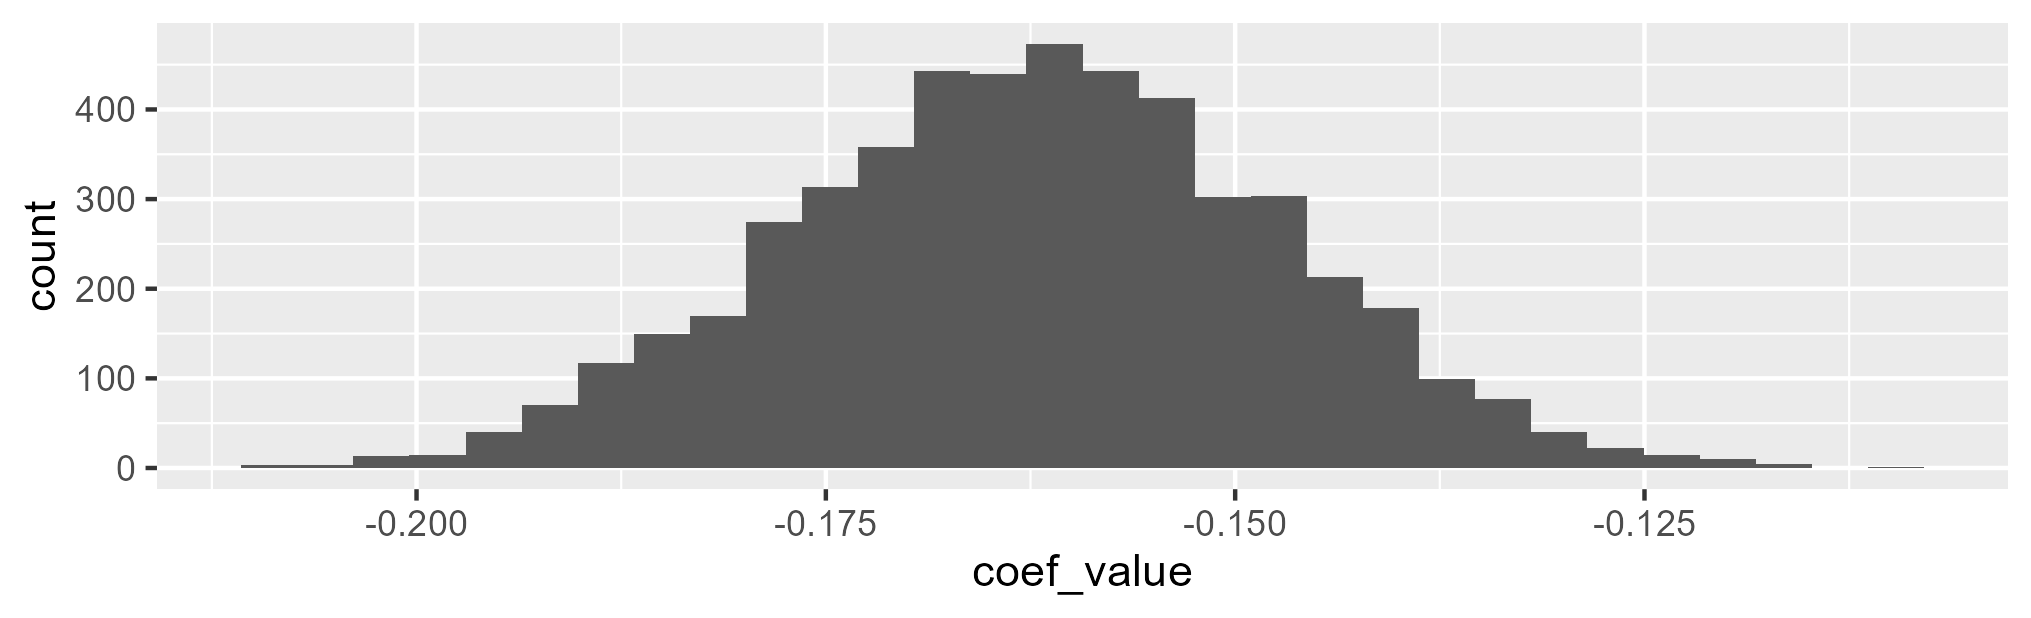
\includegraphics[scale=0.75]{../views/sd_fwl_hist.png}   
 \flushleft
 \textit{Nota:} La figura muestra el histograma de los coeficientes de $female$ obtenidos a través del bootstrap con 5000 remuestreos.
\end{figure}

La Figura \ref{fig:female} muestra la distribución del coeficiente de $female$. 
Al calcular el error estándar, obtenemos un valor de 0.01472, prácticamente idéntico al obtenido mediante la estimación por MCO.

Al estimarmos el modelo \ref{eq_inc}, no hemos considerado ningún control. Es posible que existan variables omitidas influenciando nuestros resultados. De esta manera, a fin de verificar la robustez agregamos los siguientes controles a nuestra estimación:
\begin{itemize}
    \item \textbf{Capital humano}: Incluimos edad y su cuadrado como 
    aproximación a la experiencia laboral, así como el nivel educativo más alto 
    alcanzado. Estas variables capturan diferencias en productividad potencial.
    
    \item \textbf{Intensidad laboral}: En las especificaciones con salarios 
    mensuales, se consideran las horas usuales de trabajo y la existencia de un 
    segundo empleo. En las especificaciones con salarios por hora, estas 
    variables se omiten deliberadamente para evitar un ajuste redundante.

    \item \textbf{Características del empleo}: Incorporamos ocupación, tamaño 
    de la firma, tipo de relación laboral, formalidad del empleo y la antigüedad 
    en el puesto. Estos factores permiten aproximar la comparabilidad entre 
    trabajos, tal como lo exige la noción de ``igual trabajo''.


    \item \textbf{Intensidad laboral}: En las especificaciones con salarios 
    mensuales, se consideran las horas usuales de trabajo y la existencia de un 
    segundo empleo. En las especificaciones con salarios por hora, estas 
    variables se omiten deliberadamente para evitar un ajuste redundante.
\end{itemize}

La estrategia empírica consiste en estimar primero la brecha salarial sin 
controles y, posteriormente, añadir secuencialmente los bloques de covariables. 
De este modo, se puede observar cómo evoluciona el coeficiente asociado a la 
variable de género, lo que permite interpretar en qué medida el diferencial 
incondicional se explica por diferencias observables en características de los 
trabajadores y de sus empleos. En esta parte estimamos apenas como variable dependente la variable de ingreso de la ocupación principal por hora. 
\begin{table}[!htbp] 
\centering 
\caption{Resultados de las regresiones con controles} 
\label{cuadro_controls} 
\resizebox{\textwidth}{!}{
\begin{tabular}{@{\extracolsep{5pt}}lccccc} 
\\[-1.8ex]\hline 
\hline \\[-1.8ex] 
 & \multicolumn{5}{c}{\textit{Variable dependiente:}} \\ 
\cline{2-6} 
\\[-1.8ex] & \multicolumn{5}{c}{log(y\_ingLab\_m\_ha)} \\ 
\\[-1.8ex] & (1) & (2) & (3) & (4) & (5)\\ 
\hline \\[-1.8ex] 
 female & $-$0.045$^{***}$ & $-$0.058$^{***}$ & $-$0.142$^{***}$ & $-$0.179$^{***}$ & $-$0.106$^{***}$ \\ 
  & (0.015) & (0.014) & (0.012) & (0.012) & (0.012) \\ 
  & & & & & \\ 
 age &  & 0.068$^{***}$ & 0.062$^{***}$ & 0.068$^{***}$ & 0.038$^{***}$ \\ 
  &  & (0.004) & (0.003) & (0.003) & (0.003) \\ 
  & & & & & \\ 
 age\_sqr &  & $-$0.001$^{***}$ & $-$0.001$^{***}$ & $-$0.001$^{***}$ & $-$0.0003$^{***}$ \\ 
  &  & (0.00004) & (0.00004) & (0.00004) & (0.00003) \\ 
  & & & & & \\ 
 primarios incompleto &  &  & 0.199$^{**}$ & 0.223$^{**}$ & 0.167$^{**}$ \\ 
  &  &  & (0.094) & (0.093) & (0.076) \\ 
  & & & & & \\ 
 as.factor(primario completo)4 &  &  & 0.289$^{***}$ & 0.303$^{***}$ & 0.203$^{***}$ \\ 
  &  &  & (0.091) & (0.090) & (0.073) \\ 
  & & & & & \\ 
 as.factor(secundario incompleto)5 &  &  & 0.347$^{***}$ & 0.355$^{***}$ & 0.229$^{***}$ \\ 
  &  &  & (0.091) & (0.089) & (0.073) \\ 
  & & & & & \\ 
 as.factor(secundario completo)6 &  &  & 0.565$^{***}$ & 0.575$^{***}$ & 0.292$^{***}$ \\ 
  &  &  & (0.090) & (0.088) & (0.072) \\ 
  & & & & & \\ 
 as.factor(terciario)7 &  &  & 1.253$^{***}$ & 1.238$^{***}$ & 0.557$^{***}$ \\ 
  &  &  & (0.089) & (0.088) & (0.073) \\ 
  & & & & & \\ 
 totalHoursWorked &  &  &  & $-$0.009$^{***}$ & $-$0.010$^{***}$ \\ 
  &  &  &  & (0.0005) & (0.0004) \\ 
  & & & & & \\ 
 cuentaPropia &  &  &  &  &  \\ 
  &  &  &  &  &  \\ 
  & & & & & \\ 
 microEmpresa &  &  &  &  & $-$0.392$^{***}$ \\ 
  &  &  &  &  & (0.044) \\ 
  & & & & & \\ 
 formal &  &  &  &  & 0.261$^{***}$ \\ 
  &  &  &  &  & (0.015) \\ 
  & & & & & \\ 
 Constant & 8.747$^{***}$ & 7.392$^{***}$ & 6.583$^{***}$ & 6.940$^{***}$ & 8.793$^{***}$ \\ 
  & (0.010) & (0.068) & (0.104) & (0.104) & (0.164) \\ 
  & & & & & \\ 
\hline \\[-1.8ex] 
Observations & 9,892 & 9,892 & 9,891 & 9,891 & 9,891 \\ 
R$^{2}$ & 0.001 & 0.046 & 0.335 & 0.358 & 0.576 \\ 
Adjusted R$^{2}$ & 0.001 & 0.045 & 0.335 & 0.358 & 0.572 \\ 
Residual Std. Error & 0.727 (df = 9890) & 0.711 (df = 9888) & 0.593 (df = 9882) & 0.583 (df = 9881) & 0.476 (df = 9798) \\ 
F Statistic & 9.317$^{***}$ (df = 1; 9890) & 158.028$^{***}$ (df = 3; 9888) & 623.580$^{***}$ (df = 8; 9882) & 612.986$^{***}$ (df = 9; 9881) & 144.719$^{***}$ (df = 92; 9798) \\ 
\hline 
\hline \\[-1.8ex] 
\textit{Note:}  & \multicolumn{5}{r}{$^{*}$p$<$0.1; $^{**}$p$<$0.05; $^{***}$p$<$0.01} \\ 
\end{tabular} 
} 
\end{table}

\noindent \textit{Nota:} En la ecuación (5) se omitieron las variables relacionadas con el oficio y el número de personas que trabajan en la empresa.

Los resultados en el Cuadro \ref{cuadro_controls} muestran que el coeficiente de $female$ sigue siendo negativo y significativo. Además, la inclusión de controles incrementa la magnitud del coeficiente. El modelo con todos los controles indica que las mujeres llegan a ganar aproximadamente un 10\% menos que los hombres, dado que ambos tengan la misma experiencia, edad y ejerzan profesiones similares.

Un aspecto interesante sería estimar la edad pico en la que las mujeres alcanzarían su máximo salarial. Esto puede calcularse mediante un problema sencillo de maximización: 
\[
pico = -\frac{\beta_2}{2\beta_3},
\] 
donde $\beta_2$ es el coeficiente de \textit{age} y $\beta_3$ es el coeficiente de \textit{age}$^2$.

\begin{figure}[H]
\caption{Edad pico según nuestros modelos} \label{fig:age_peak_bar}
    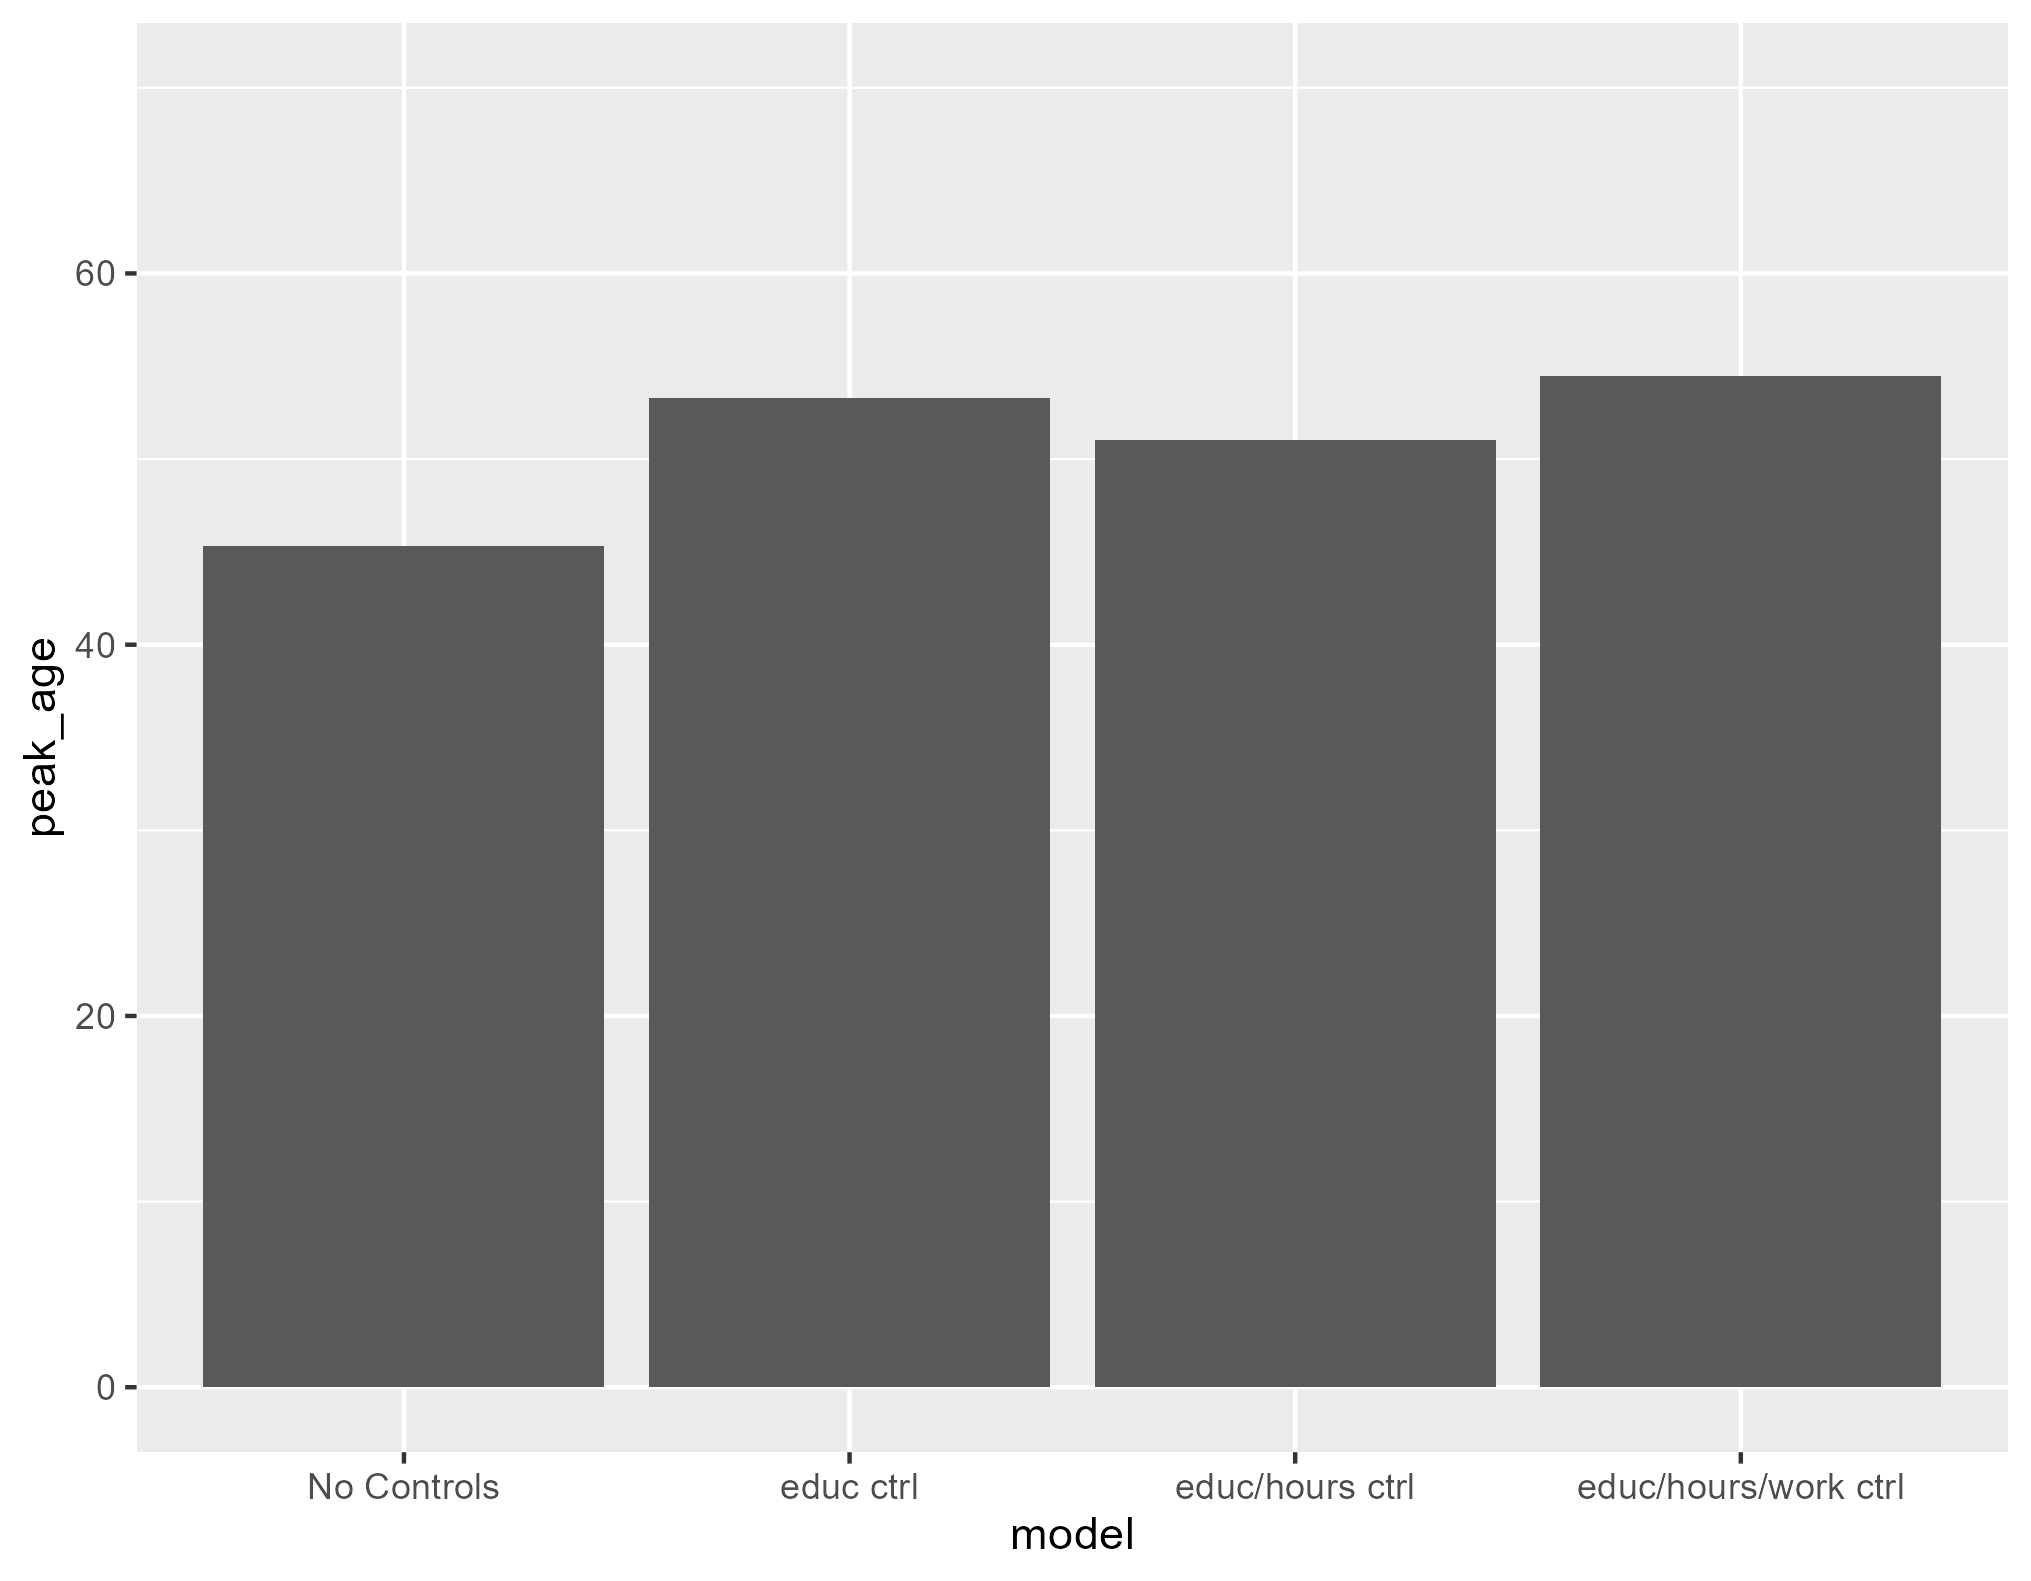
\includegraphics[scale=0.75]{../views/age_peak_bar.png}   
 \flushleft
\end{figure}

La Figura \ref{fig:age_peak_bar} muestra los resultados de la edad pico. En general, los modelos indican que la edad pico estaría entre los 45 y 54 años. La inclusión de controles parece incrementar dicha edad. Cabe señalar que, al estimar la edad pico a partir de los coeficientes de MCO, no es posible calcular sus errores estándar ni los intervalos de confianza. Para generar dichos intervalos, empleamos el método bootstrap. En particular, remuestreamos los datos 2000 veces y registramos la distribución de la edad pico. Con esta distribución construimos el intervalo de confianza al 5\% para nuestros modelos.

\begin{figure}[H]
\caption{Intervalos de confianza de la edad pico} \label{fig:age_whiskey_bar}
    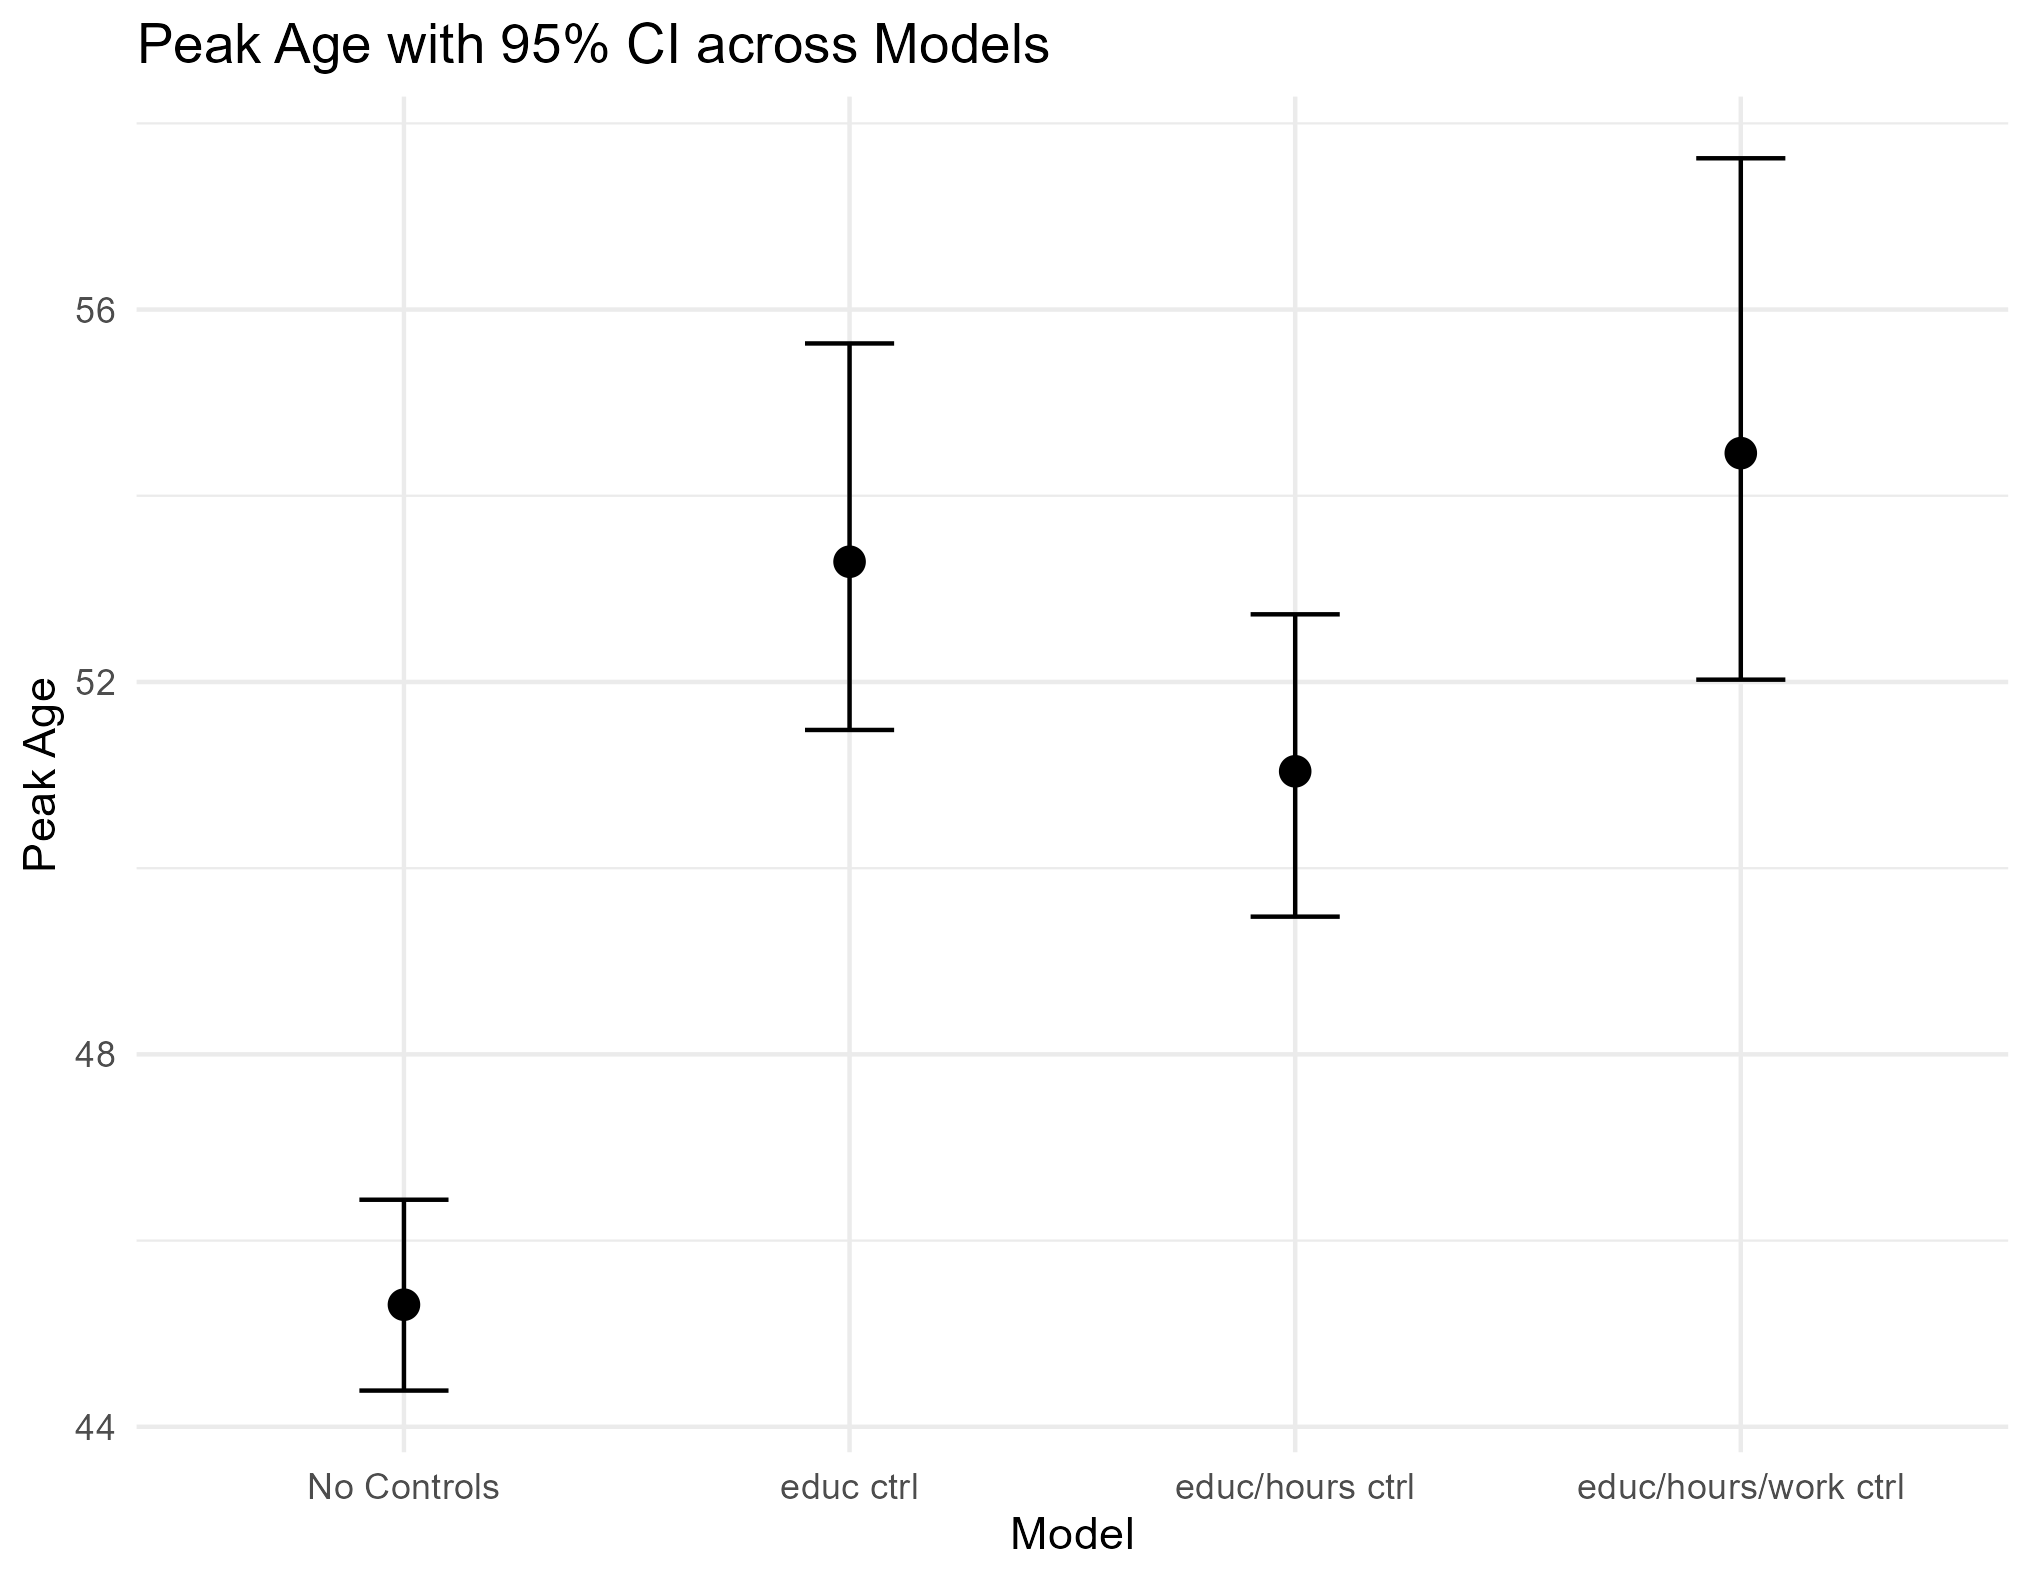
\includegraphics[scale=0.75]{../views/age_whiskey_point.png}   
 \flushleft
\end{figure}

La Figura \ref{fig:age_whiskey_bar} muestra los resultados de los intervalos de confianza. Como era de esperar, la inclusión de más controles amplía dichos intervalos; sin embargo, el incremento no supera los 2 años con respecto al valor central de la estimación.
\section{Results}

Referencing tables is very easy you can do the following: In Table \ref{tab:avdiscriminationrates} ...

Citing papers is easier, for example \cite{albouy2020unlocking} shows that crime around parks. For many papers in parenthesis \cite{albouy2020unlocking,mcmillen2019more} 

\subsection{Robustness}
\section{Conclusion}





%%%%%%%%%%%%%%%%%%%%%%%%%%%%%%%%%%%
%		  References				  %
%%%%%%%%%%%%%%%%%%%%%%%%%%%%%%%%%%%

\pagebreak
\singlespacing
\bibliography{References.bib}
\pagebreak


%%%%%%%%%%%%%%%%%%%%%%%%%%%%%%%%%%%
%		  TABLES				  %
%%%%%%%%%%%%%%%%%%%%%%%%%%%%%%%%%%%
\section*{Tables and Figures}


\begin{table}[H]                                 
\footnotesize \centering                                 \begin{threeparttable}                                 \captionsetup{justification=centering}                      \caption{Overall Response Rates }                               \label{tab:avdiscriminationrates}                               \begin{tabular}{@{\extracolsep{5pt}} lcc}                       \\[-1.8ex]\hline                                  
\hline \\[-1.8ex]                                  & \multicolumn{2}{c}{\it Dependent variable:} \\                                 & \multicolumn{2}{c}{\it  Response} \\                                 \cline{2-3}\\ [-1.8ex]        
                    &\multicolumn{1}{c}{(1)}   &\multicolumn{1}{c}{(2)}   \\
\hline
Minority            &     -0.323***&               \\
                    &(-0.213,-0.412)   &               \\
African American    &               &     -0.432***\\
                    &               &(-0.312,-0.532)   \\
Hispanic/LatinX     &               &     0.7027\\
                    &               &(-0.670,0.818)   \\
\hline
 Mean Response (White)&        0.4   &        0.4   \\
\hline Gender       &         Yes   &         Yes   \\
Education Level     &         Yes   &         Yes   \\
Inquiry Order       &         Yes   &         Yes   \\
\hline Observations &      45,202   &      45,202   \\
\\[-1.8ex]\hline                          
\hline \\[-1.8ex]           
\end{tabular}      
\begin{tablenotes}[scriptsize,flushleft] 
\scriptsize                         
\item Notes: Table reports coeficients from a within-property linear regression model including controls for gender, education and order the inquiry was sent. Standard errors clustered at the CBSA Downtown/Suburb level. 90\% confidence intervals reported in parentheses.                        
\end{tablenotes}                         
\end{threeparttable}                         
\end{table}        
%

\pagebreak

\begin{figure}[H]
\caption{US Map} \label{fig:robust}
    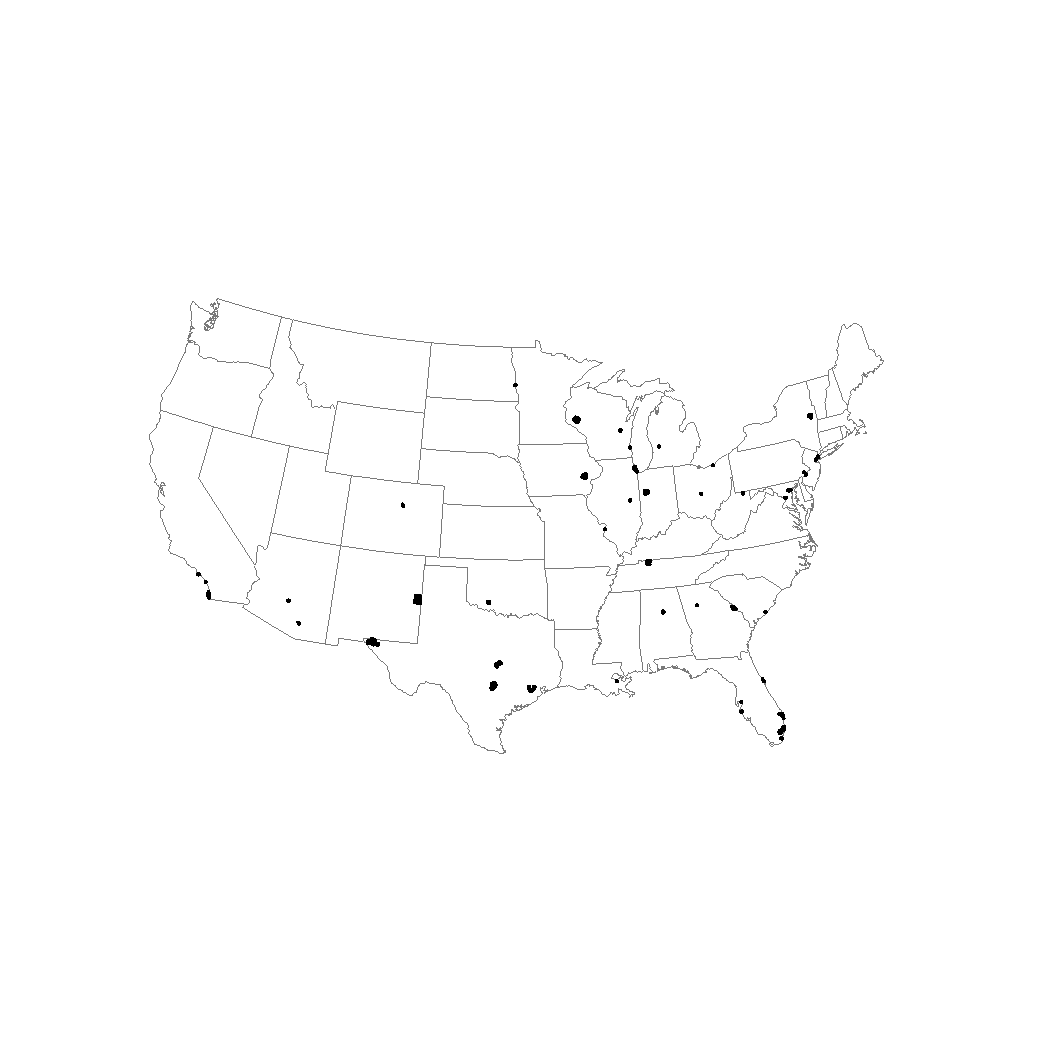
\includegraphics[scale=0.75]{../views/fig1a.pdf}   
 \flushleft
 Note: This figure shows ...
\end{figure}

%%%%%%%%%%%%%%%%%%%%%%%%%%%%%%%%
%   APPENDIX	 Tables	        %
%%%%%%%%%%%%%%%%%%%%%%%%%%%%%%%%
\pagebreak
\appendix
\renewcommand{\theequation}{\Alph{chapter}.\arabic{equation}}

\setcounter{figure}{0}
\setcounter{table}{0}
\makeatletter 
\renewcommand{\thefigure}{A.\@arabic\c@figure}
\renewcommand{\thetable}{A.\@arabic\c@table}

\section{Appendix: Tables and Figures}\label{sec:appendix_tables} 

\end{document}
